\section{Metal Camp}

\tweet{6:26PM Jul 31, 2009}{Camp opened for business by JMF/AJ! Only 3 tacklesac each from traverse chamb. Water issues - need to rig one of the damp pitches.}

The plan for \passage{Metal Camp} is an extremely light weight 2 man camp. We have an old Vango geodesic 2+ man tent whose fly was long ago eaten by UV, but which can be pitched free standing with just two of its poles. Our stoves will be the standard super safe (super slow) Tranjas. Our pits will be made up with 10mm carry mats, Vango Nitestar 450s (cheapest, warmest, synthetics we could find), buffalo bags (100\% polyester) and fleece liners (from sponsorship by Polartec back in 1996). Of course, the essential component is the Ghetto Blaster, which is an MP3 player which takes SD cards and 4AA batteries.

\name{Jarvist Frost}


\tweet{3:34PM Aug 4, 2009}{JKP/DG 2 day camp,discovered underground river at ~380m below Dark Tranquility.Leads multiplying...AJ/MF on camp night train.Much surf work.}



\begin{pagefigure}
      \checkoddpage \ifoddpage \forcerectofloat \else \forceversofloat \fi
    \centering
    \begin{subfigure}{0.49\textwidth}
        \frame{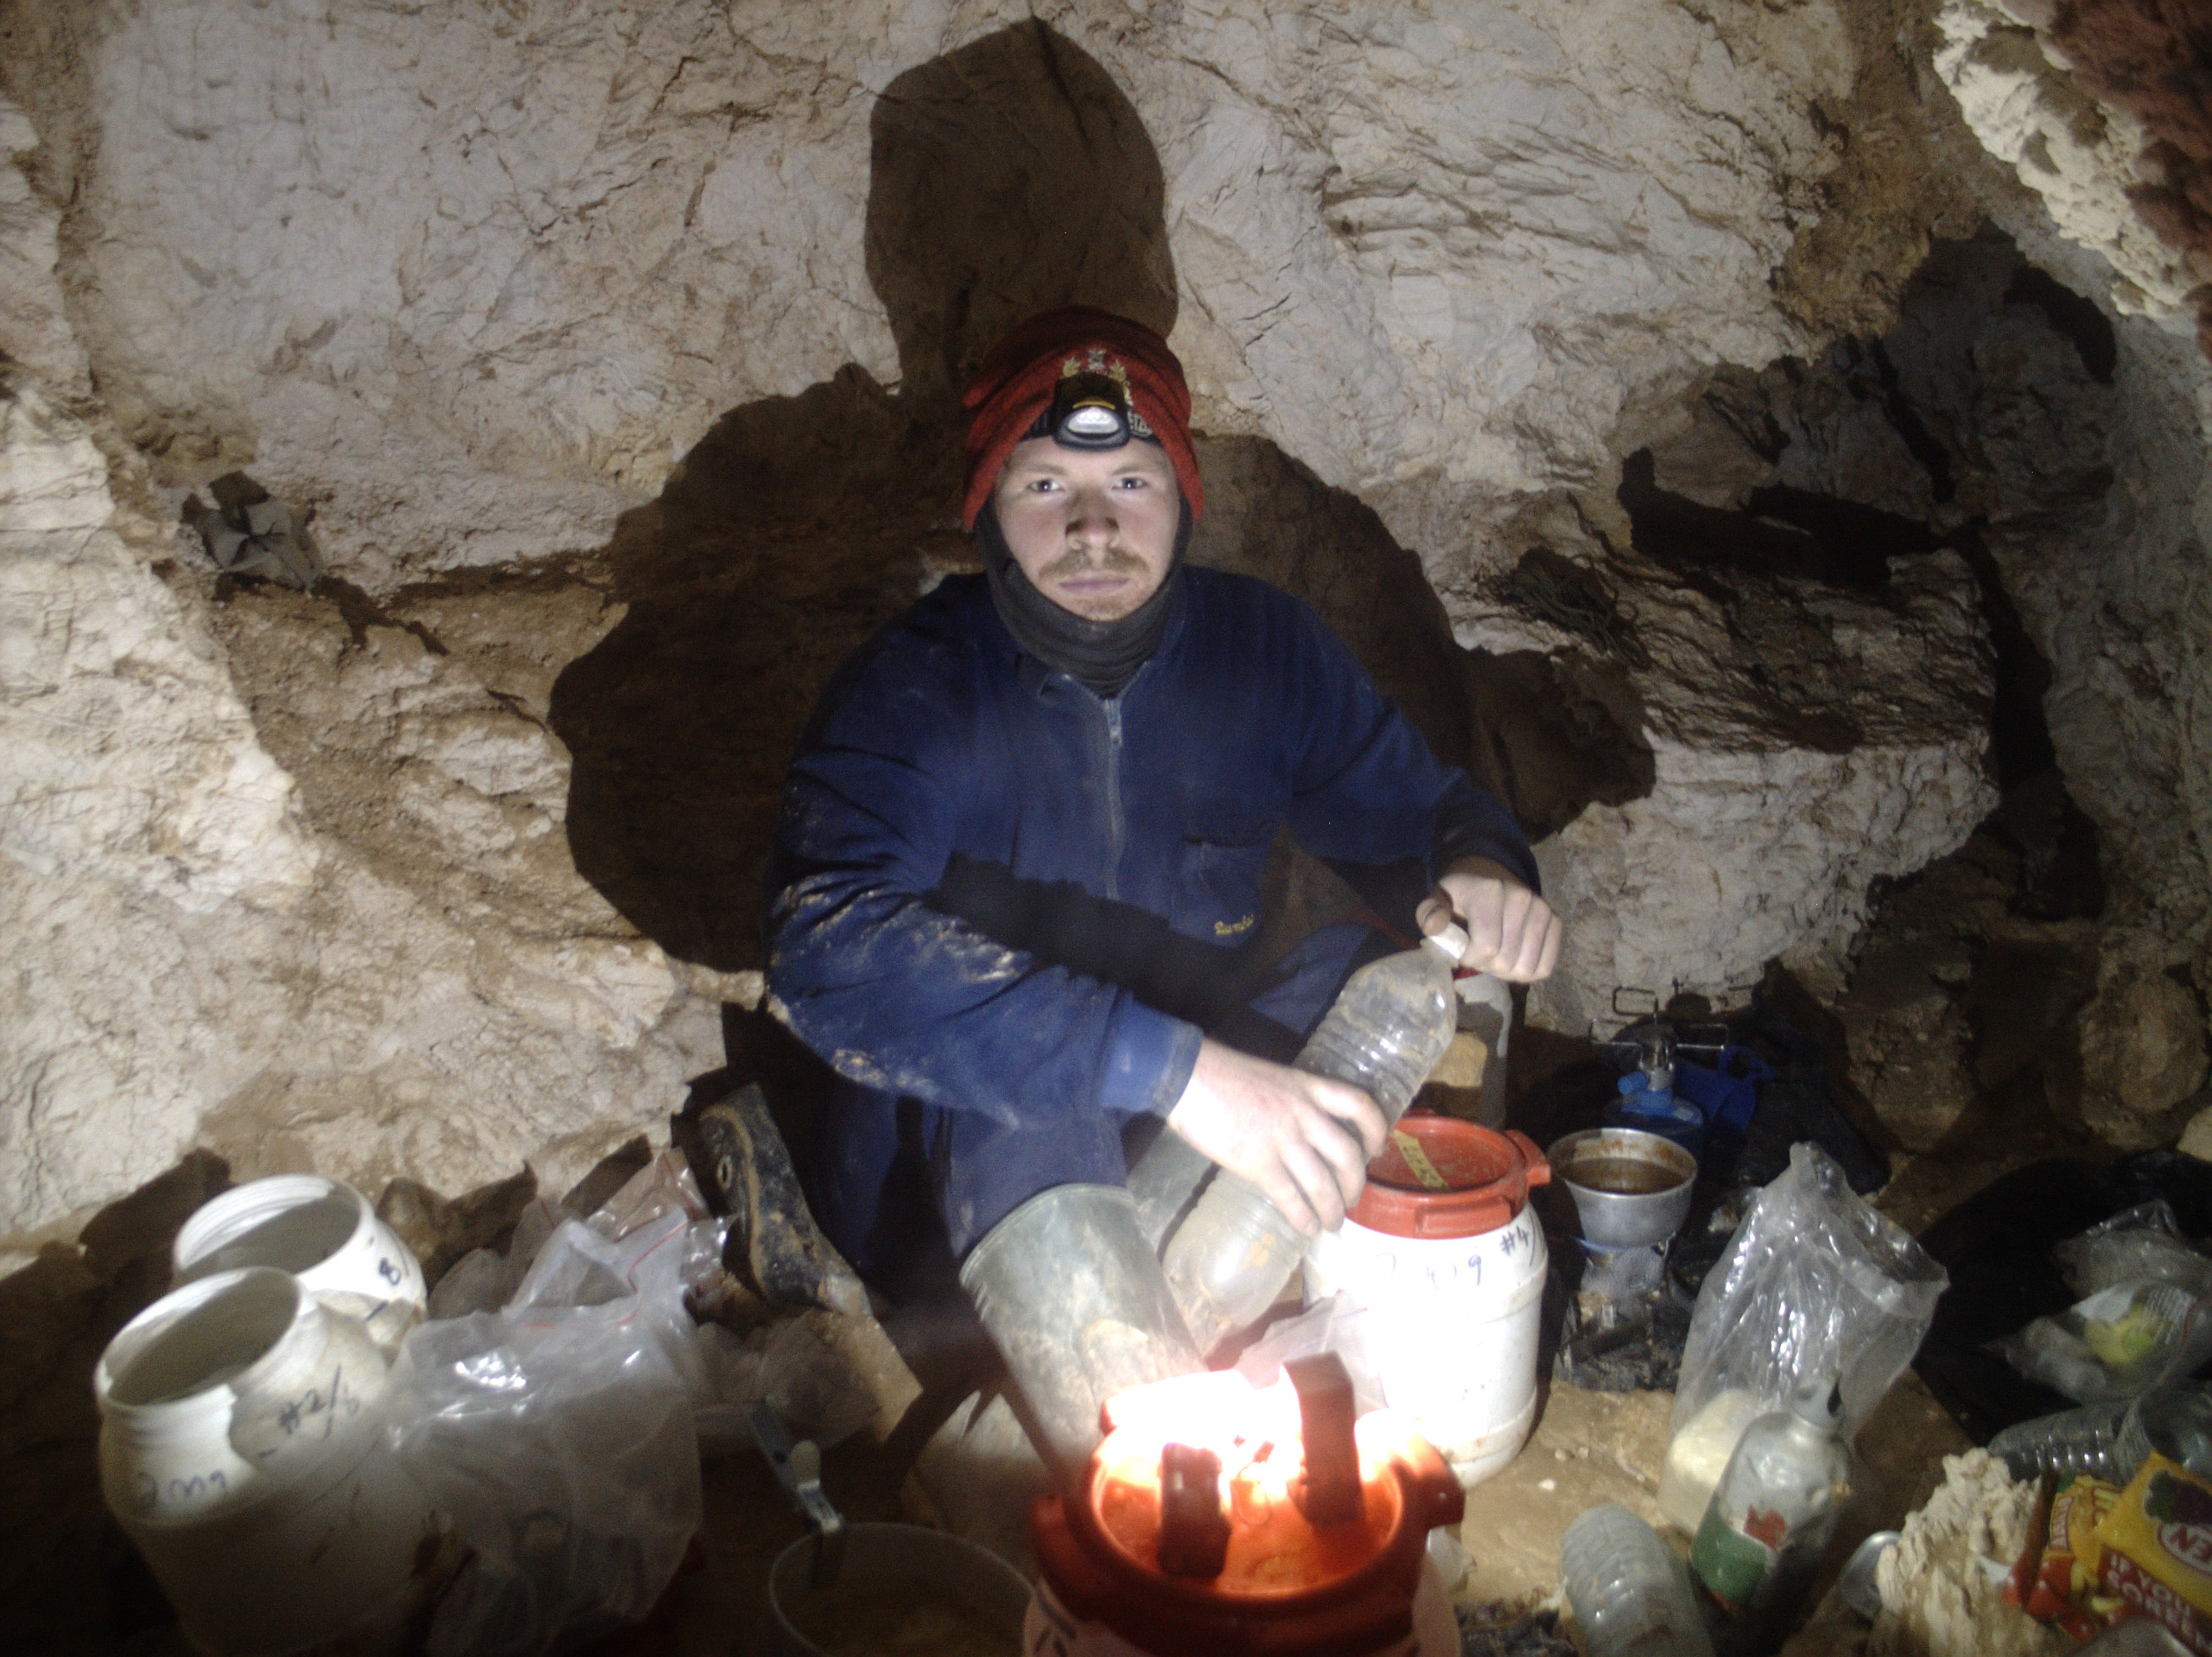
\includegraphics[width=\linewidth]{2009/logbook/2009-08-05-20.35.38 - Jarvist Frost - Canon Powershot G5 - Mike in camp by LED light staying still--orig.jpg}}
        \caption{}
    \end{subfigure}
\hfill
    \begin{subfigure}{0.49\textwidth}
    \centering
        \frame{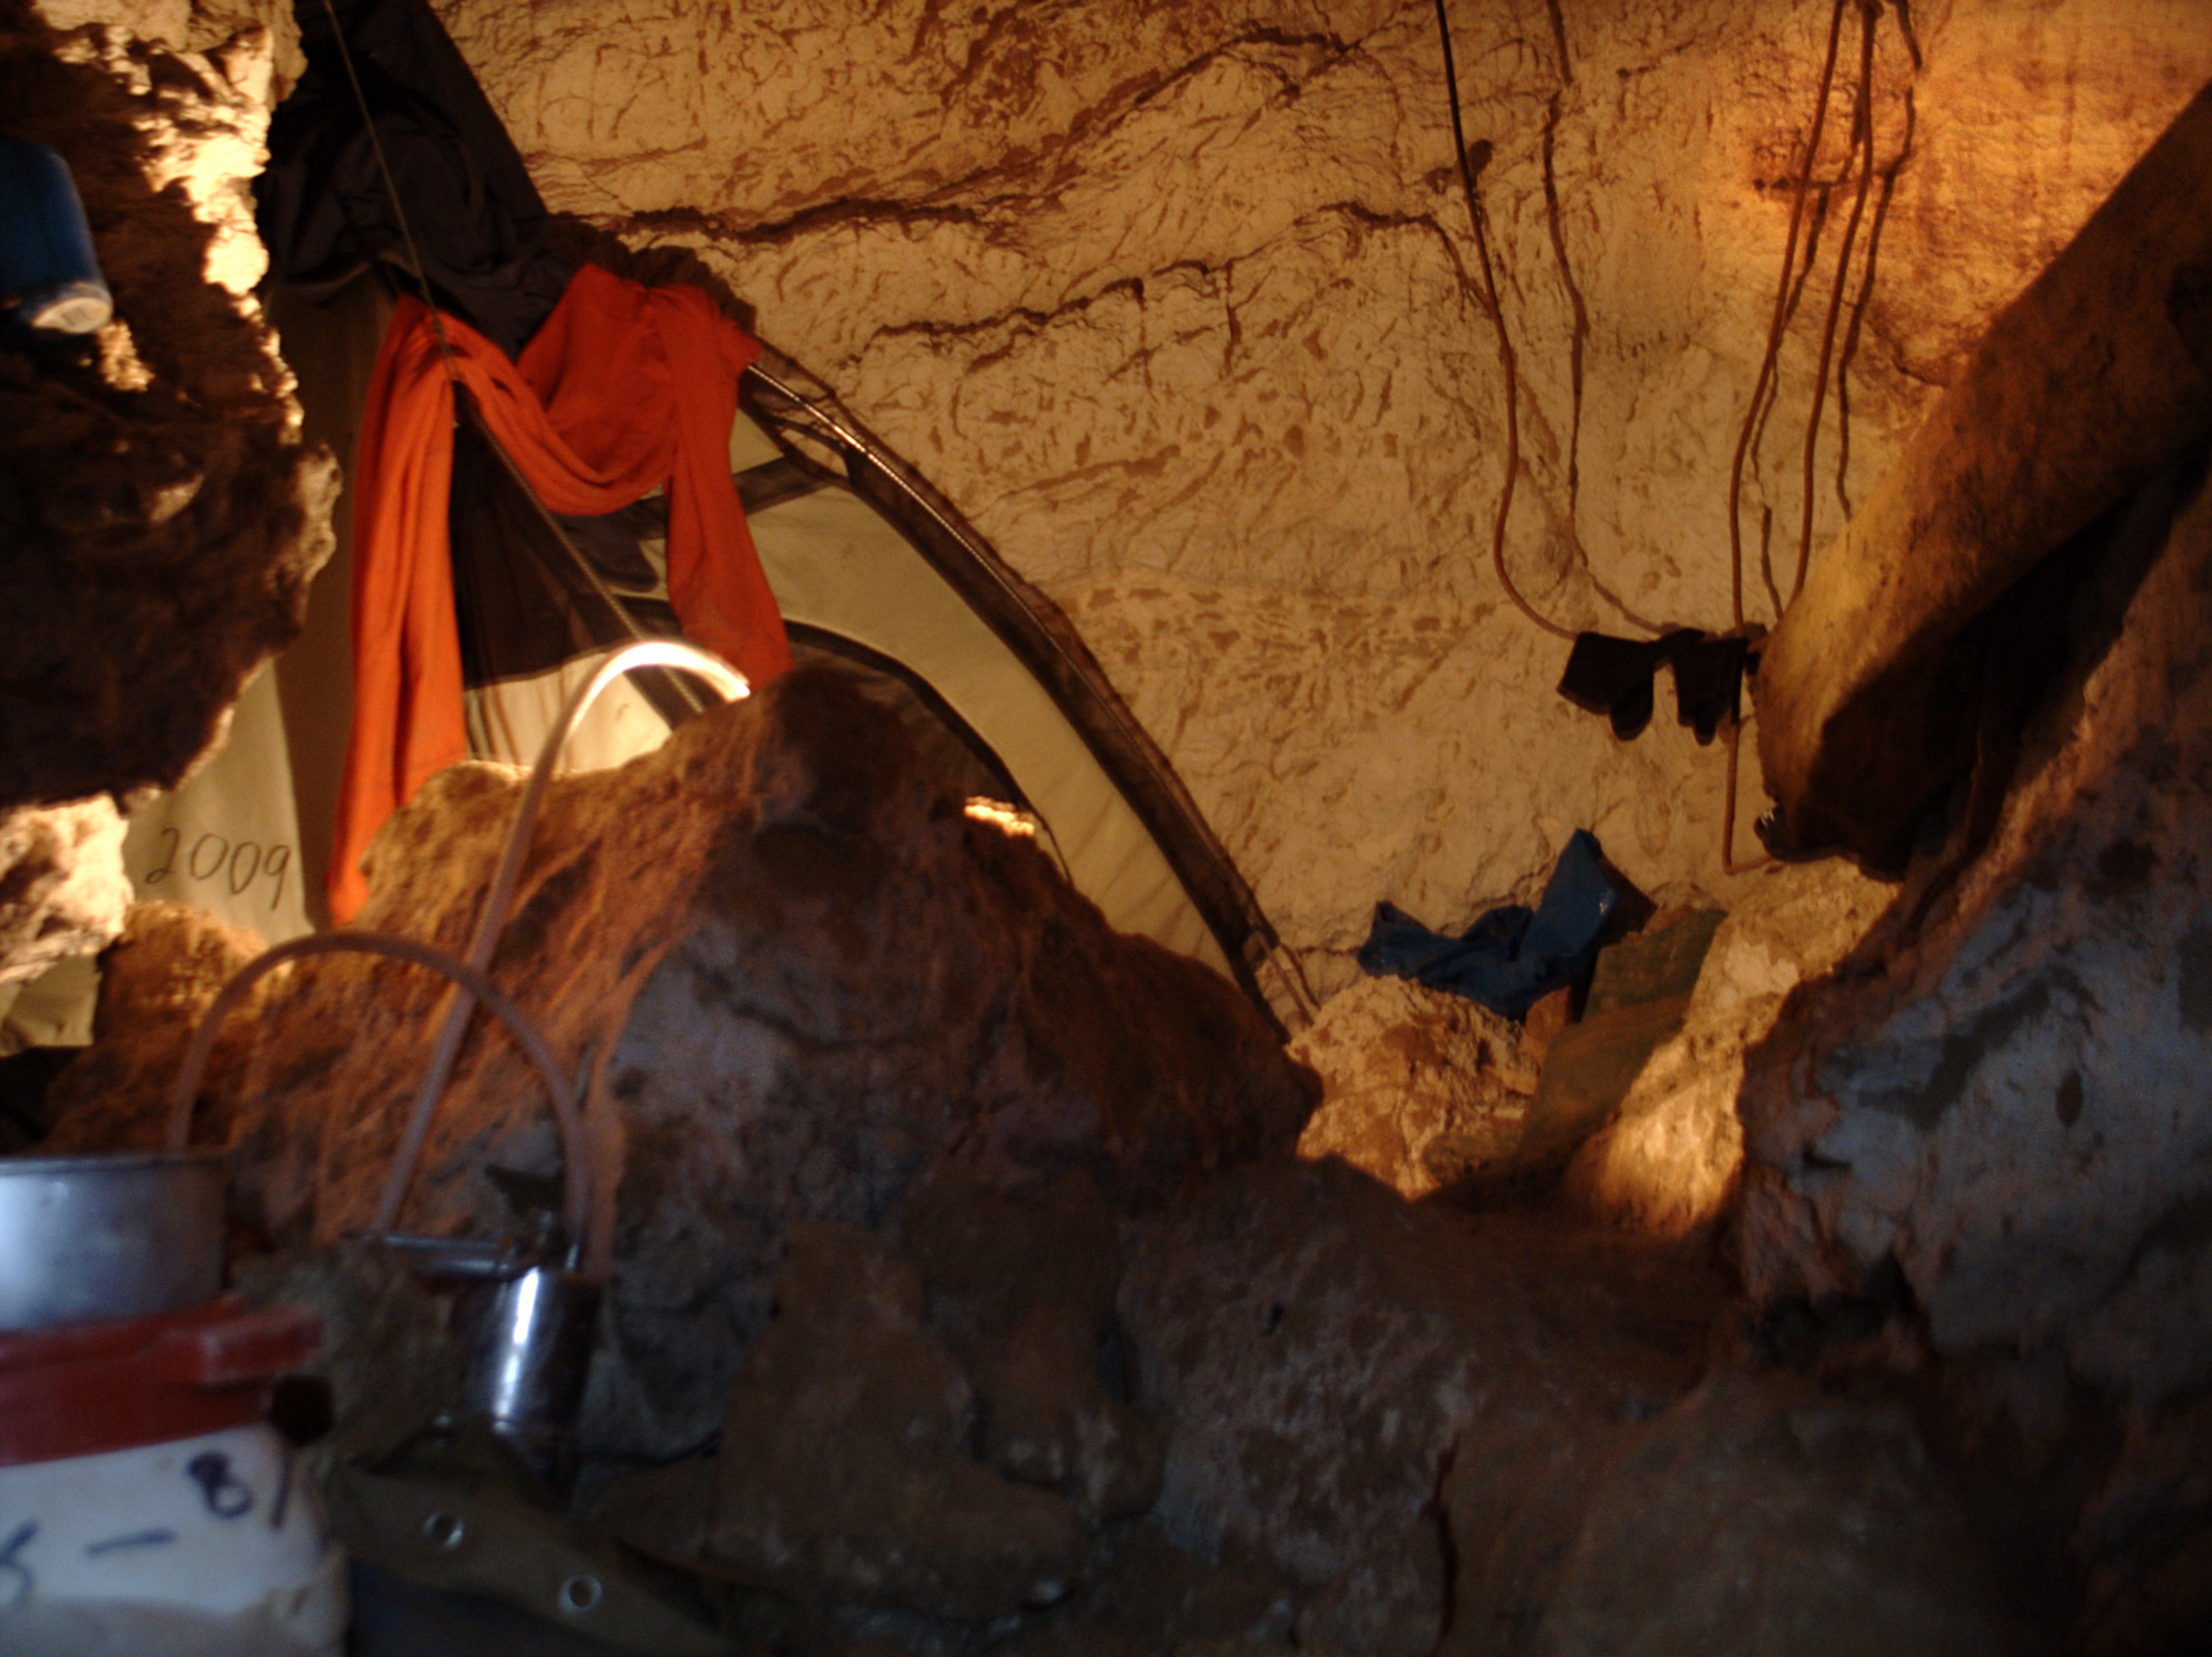
\includegraphics[width=\linewidth]{2009/logbook/2009-08-11-02.04.48 - Jarvist Frost - Canon Powershot G5 - Metal Camp by Carbide light with Gergely--orig.jpg}}
        \caption{}
\end{subfigure}
\caption{The difference that light source makes underground. \textit{(a)} Camp by LED light, cooler and whiter in colour. \textit{(b)} Camp by carbide light, warmer and more orange in colour. \pic{Jarvist Frost}}
\end{pagefigure}


\begin{pagefigure}
\checkoddpage \ifoddpage \forcerectofloat \else \forceversofloat \fi
\frame{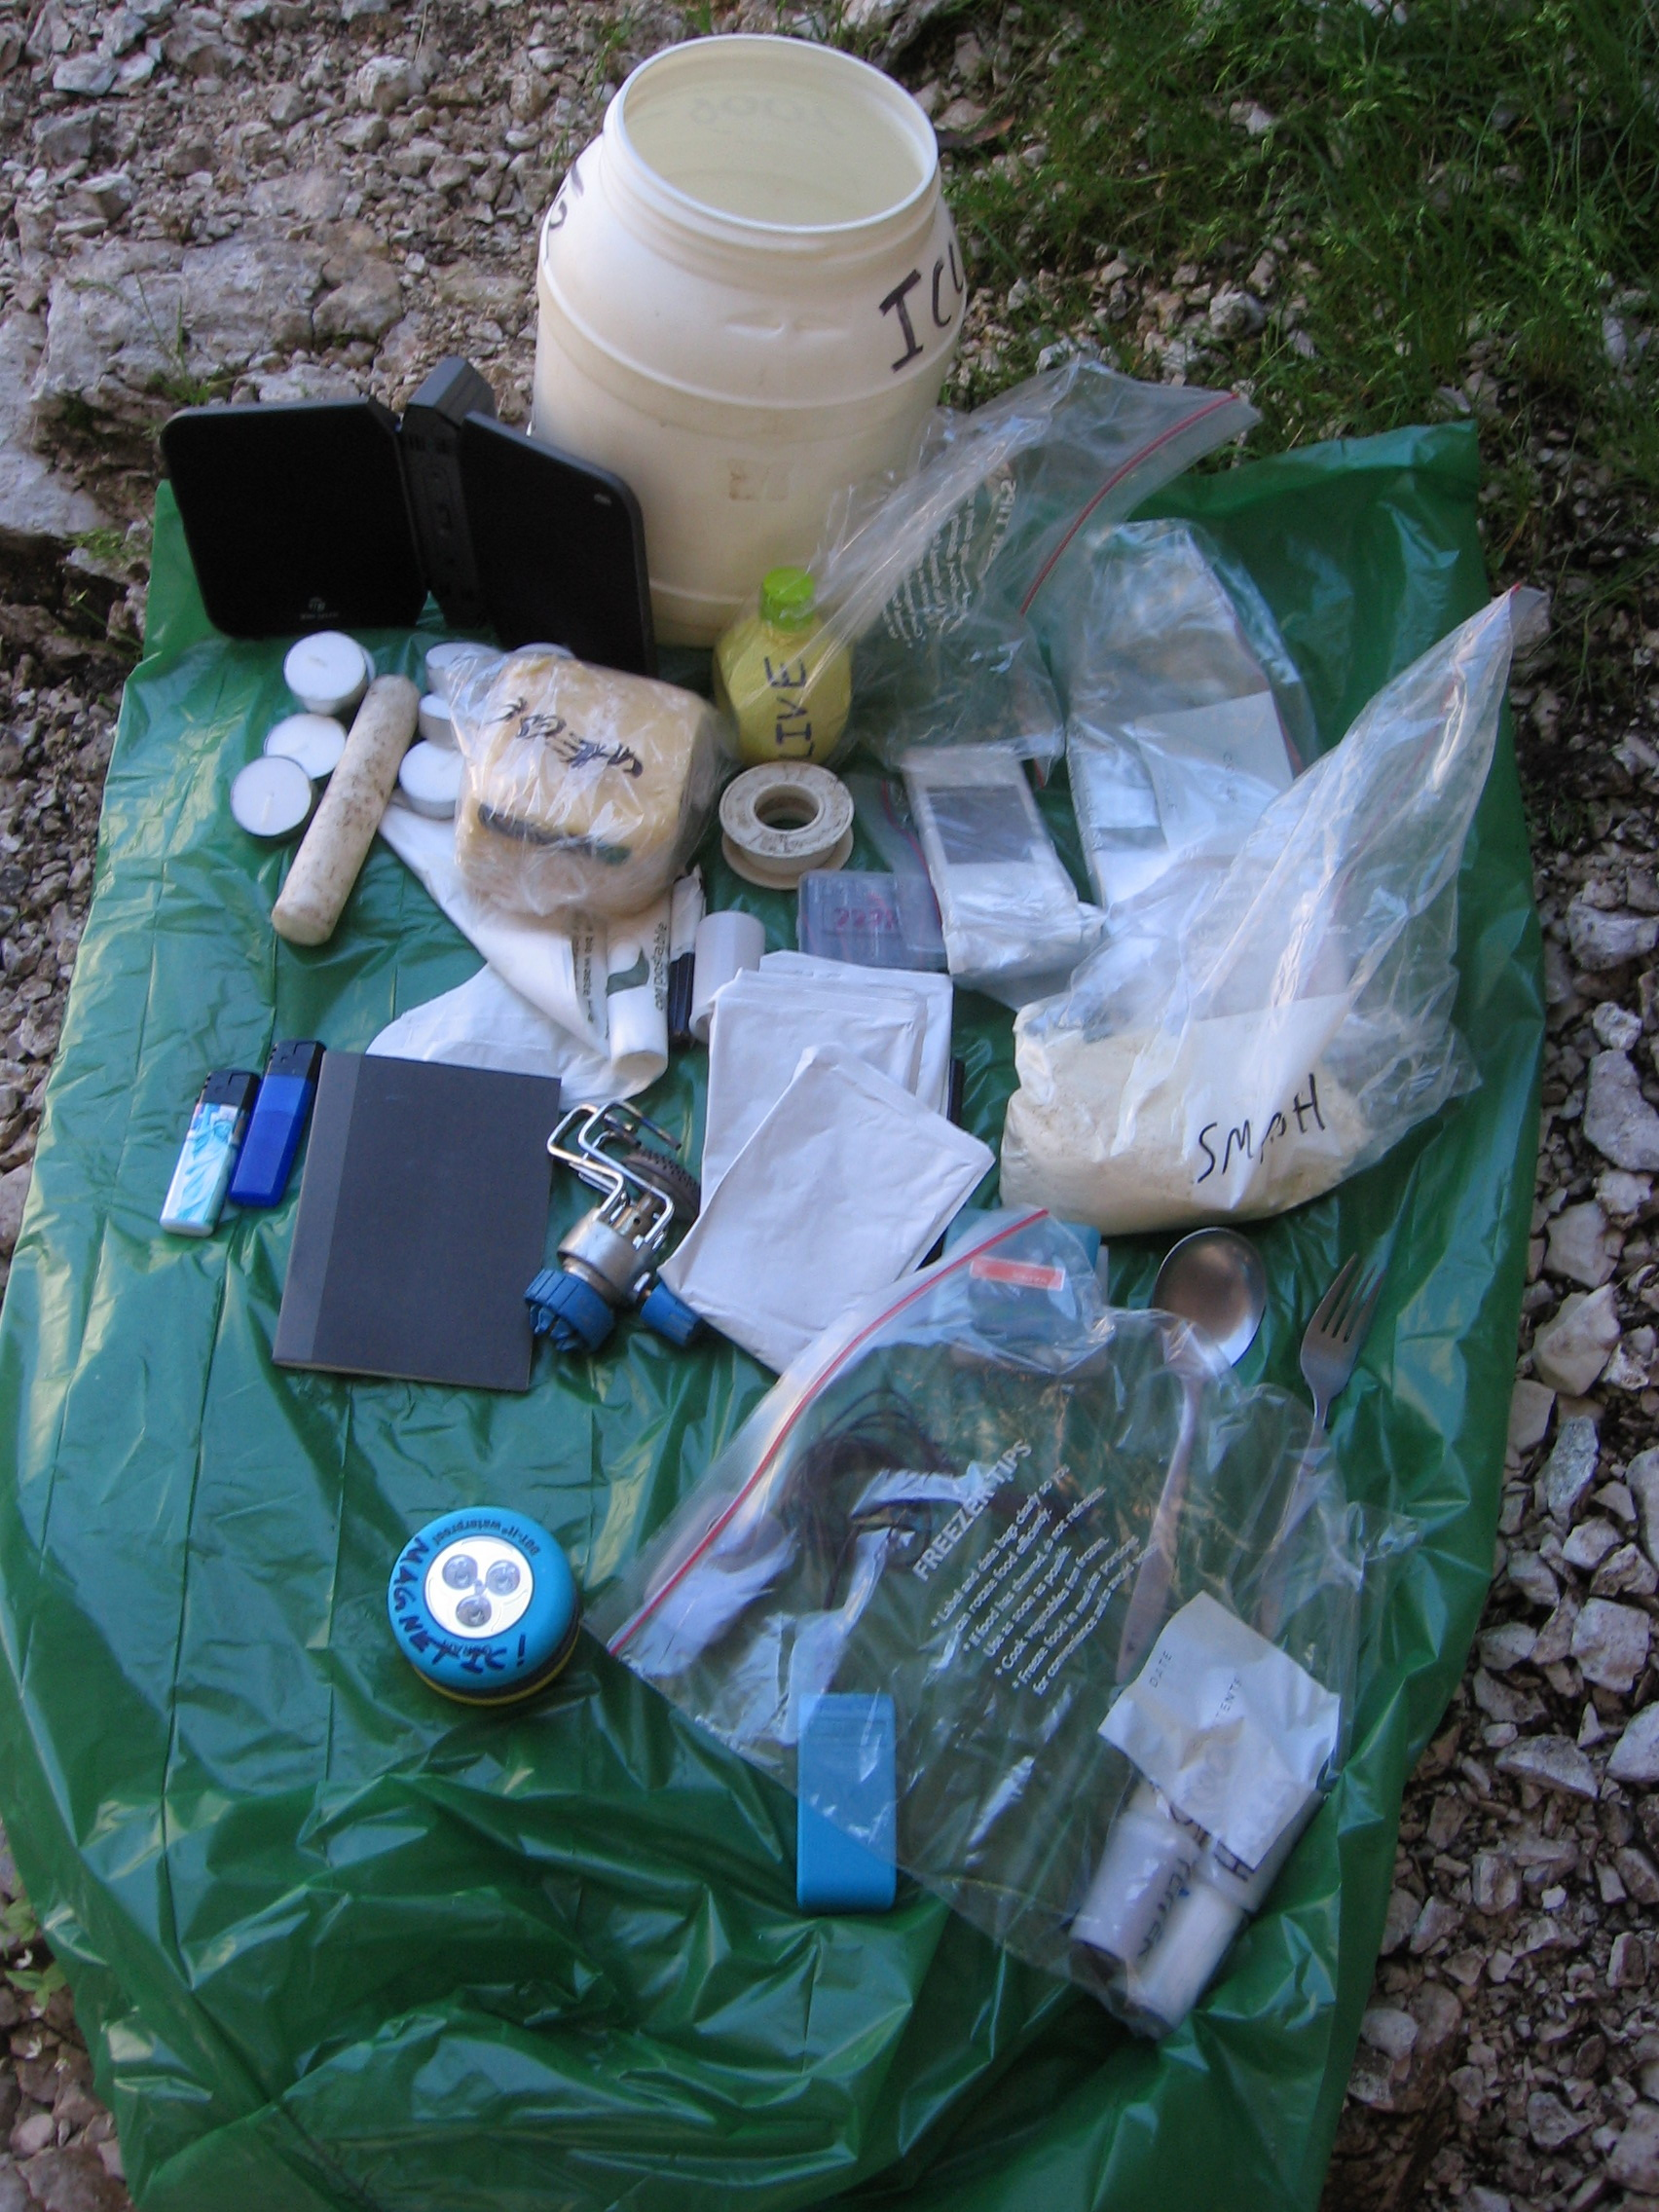
\includegraphics[width=\linewidth]{2009/logbook/2009-07-30-14.36.30 - Jarvist Frost - Canon Powershot A520 - First drum to go to underground camp2--orig.jpg}}
\caption{The first Daren drum for \passage{Metal Camp}: \textit{top to bottom, left to right} Speakers, Daren drum, tealights, candle, cheese, olive oil (in freezer bag), tape, ??, poo bags, pen??, film canister, batteries, 2 lighters, UG camp logbook, stove burner, soup sachets,  smash (potato flakes), AA batteries and cases, LED light (Osram DOT-it), headphones, cutlery, grey mp3 player, blue thing with wire to mp3??, cooking spices (pepper, salt, herbs) in freezer bag \pic{Jarvist Frost}} \label{metal camp drum}
\end{pagefigure}




\subsection{30--31 July - Andy and Jarv - The first one}

Two heavy sacks from the surface, picked up 4 comf sacks at the
\passage{Traverse Chamber}. Passed through squeezes with the aid of the handl
? Cord. \passage{Something fishy} was a bit of a campsite - but only room for one
pit. Dumped sacks and continued to look for greener pasteures\ldots{} and
refound here! Looked very nice at first -- a few drips, flat, dry-ish
mud. Moved rocks and set a tent -- the place not looked so good, bit of
a quagmire? Found 1,5L of water in \passage{Something Fishy} -- drips
provided about 5 mL overnight.

So \passage{Dangermouse}/drips on \passage{Kill'em All} way have to be the way
forward\ldots{}
\name{Jarvist Frost}



\newpage


\begin{pagefigure}
	\checkoddpage \ifoddpage \forcerectofloat \else \forceversofloat \fi
	\centering
	
   	\begin{subfigure}[t]{0.49\textwidth}
    	\centering
     	\frame{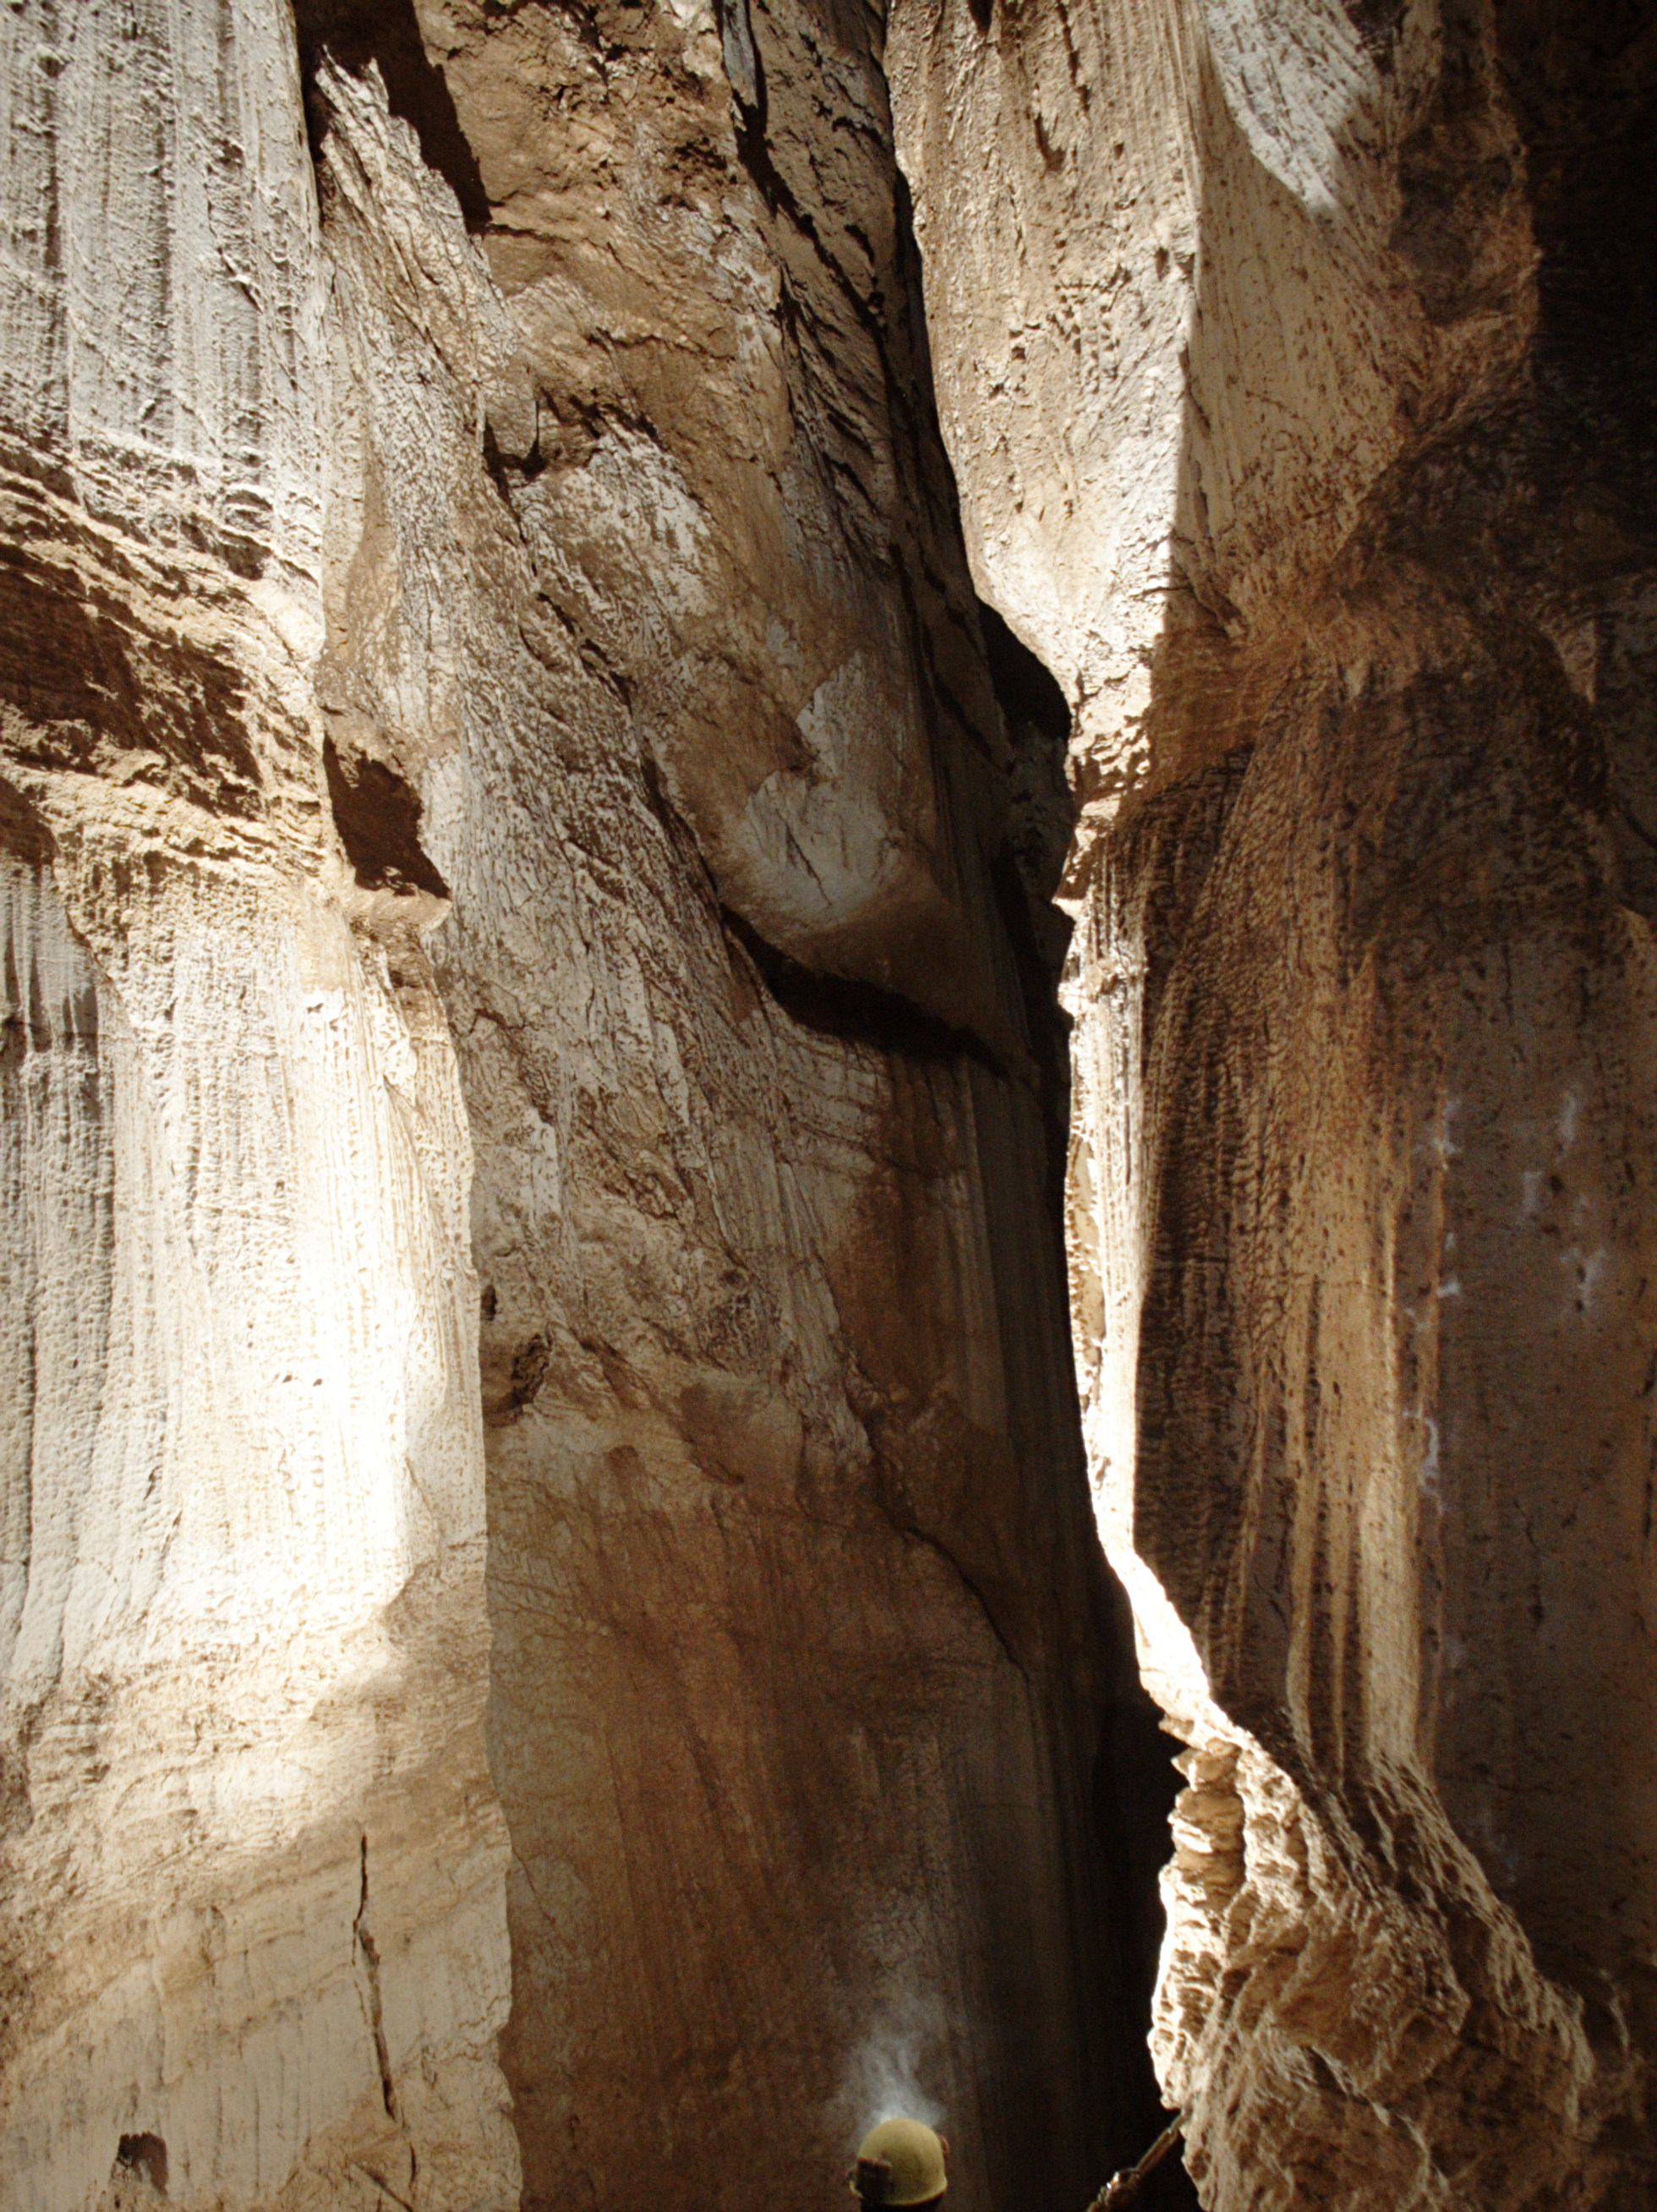
\includegraphics[width=\linewidth]{2009/logbook/2009-08-10-18.49.50 - Jarvist Frost - Canon Powershot G5 - mirage canyon - upper shot--orig.jpg}}
       	\caption{} \label{mirage canyon}
    \end{subfigure}
    \hfill
	\begin{subfigure}[t]{0.49\textwidth}
		\centering
		\frame{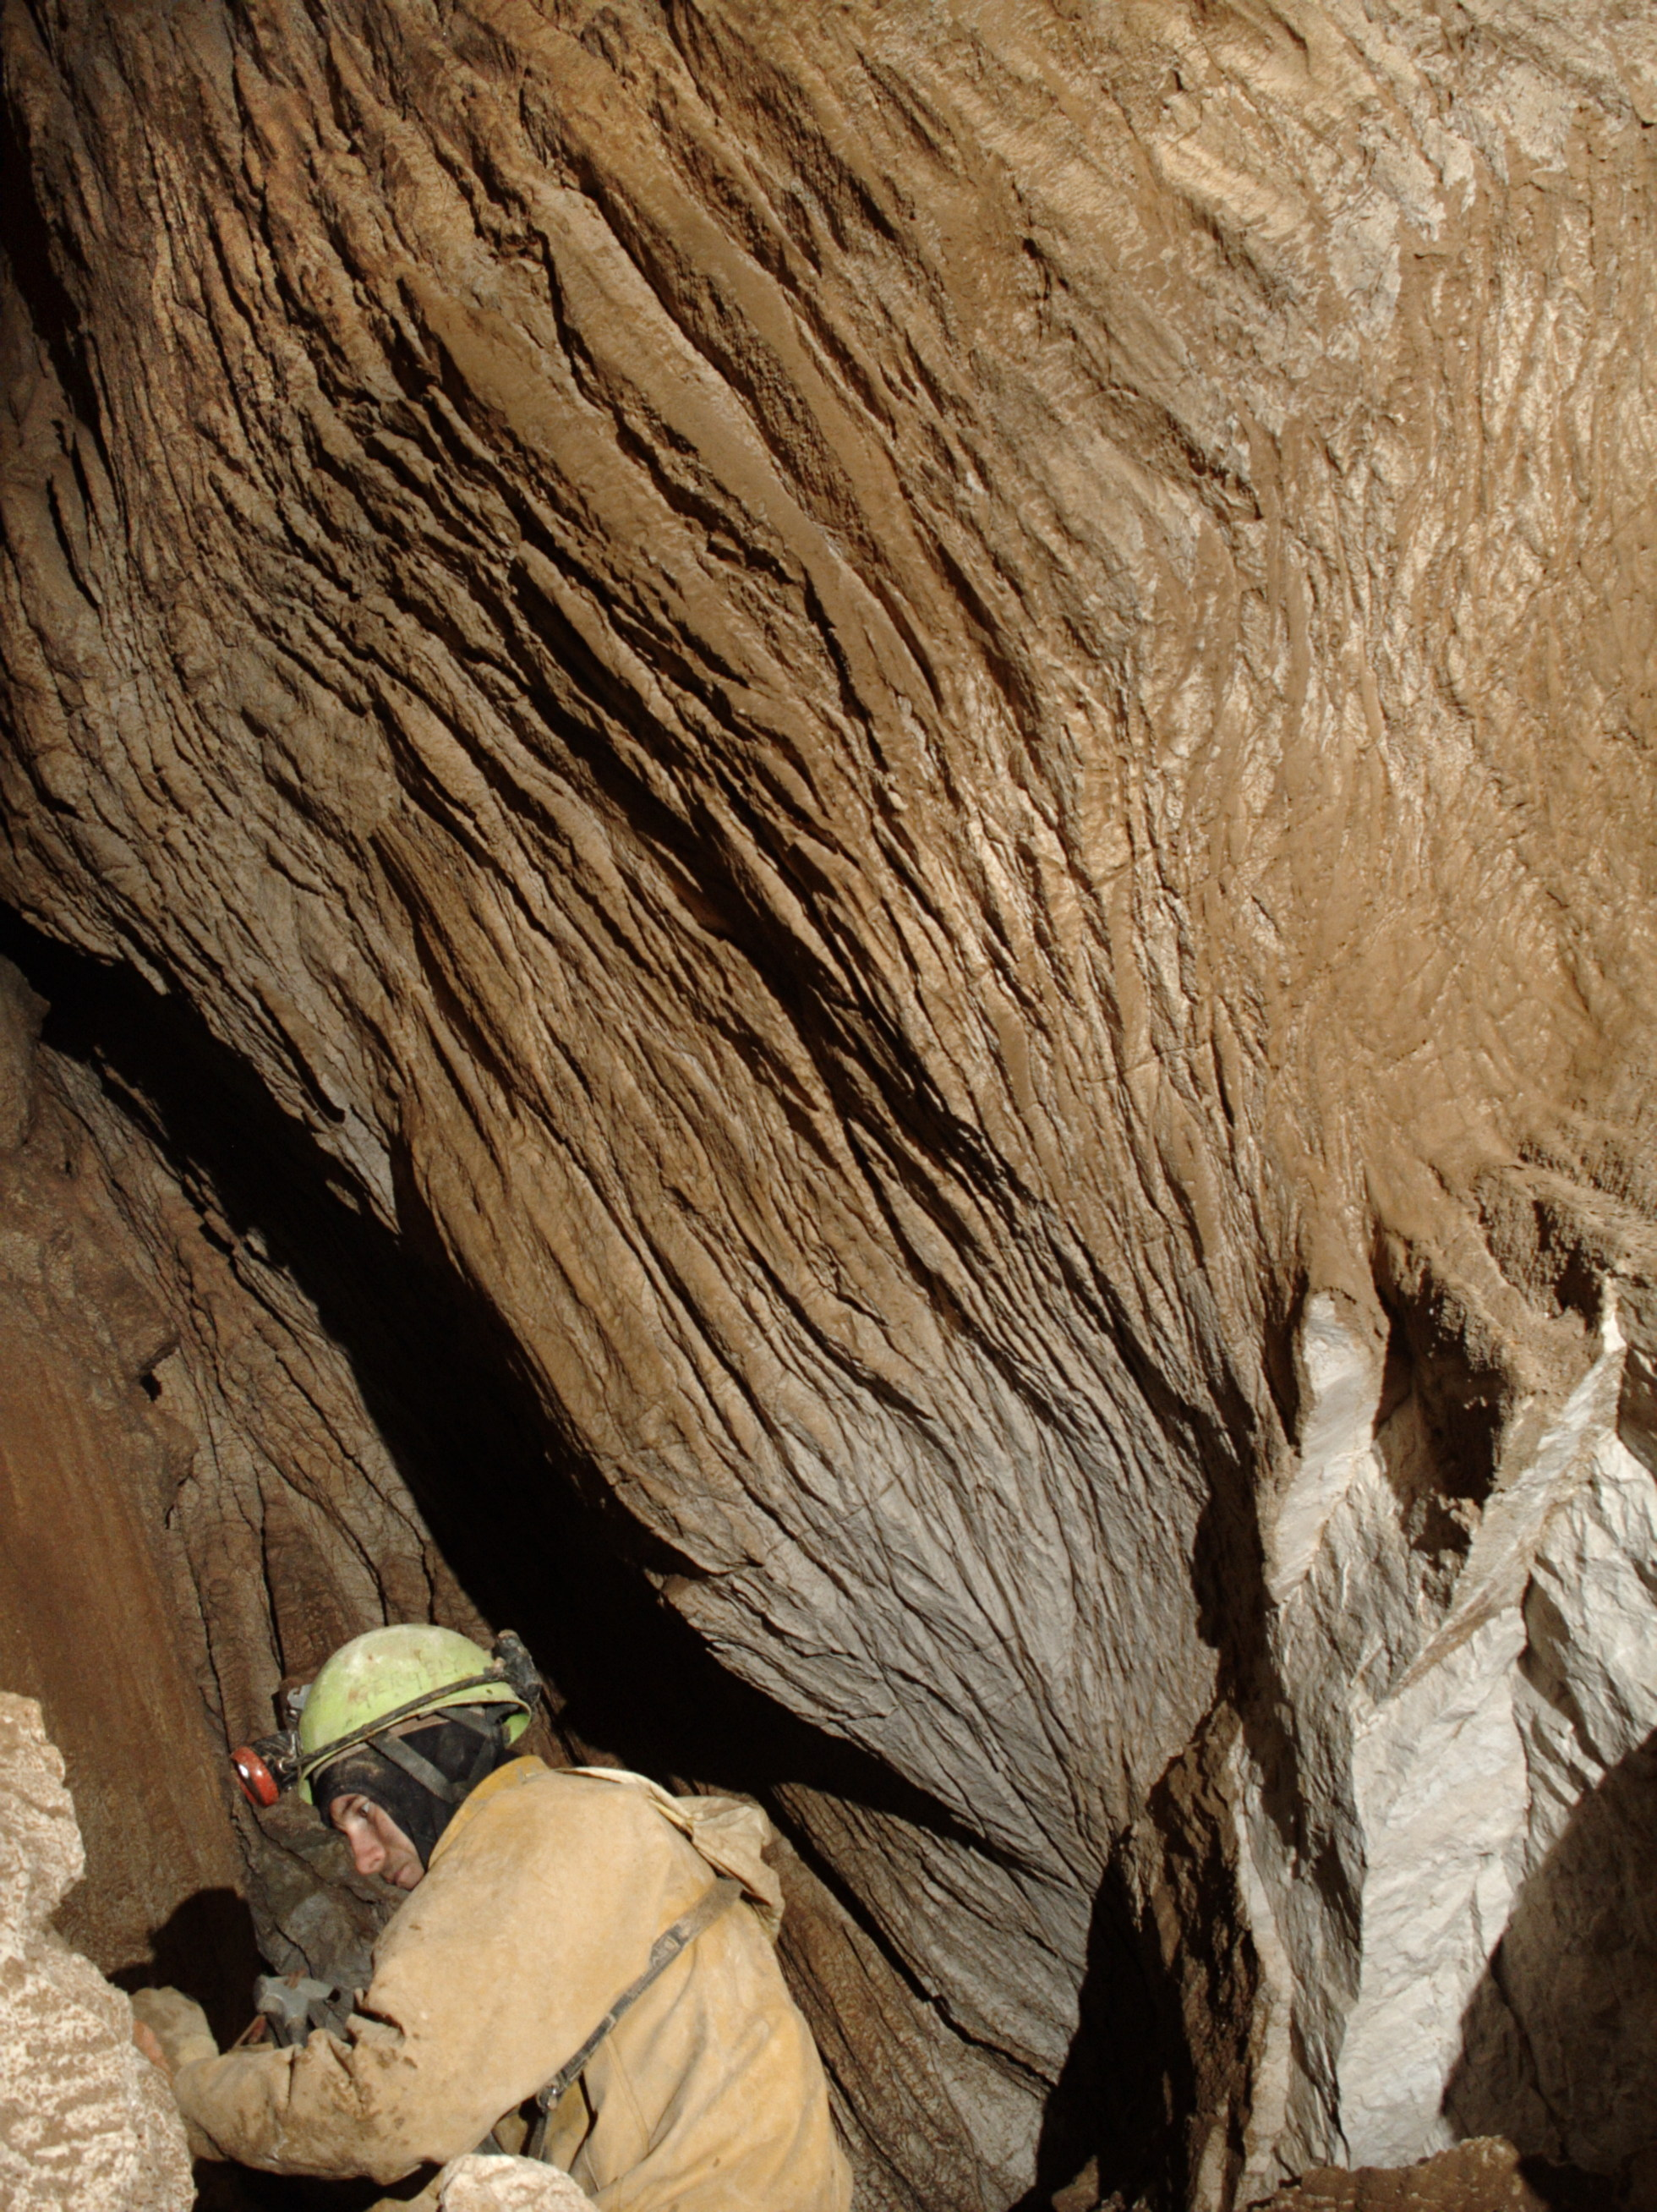
\includegraphics[width=\linewidth,]{2009/logbook/2009-08-10-19.40.48 - Jarvist Frost - Canon Powershot G5 - 2 minutes to midnight - gergely bolting traverse limestone fluting--orig.jpg}}
		 \caption{}\label{gergely 2 minutes fluting}
	\end{subfigure}
    \vspace{0cm}
	
	\begin{subfigure}[h]{\textwidth}
		\centering
		\frame{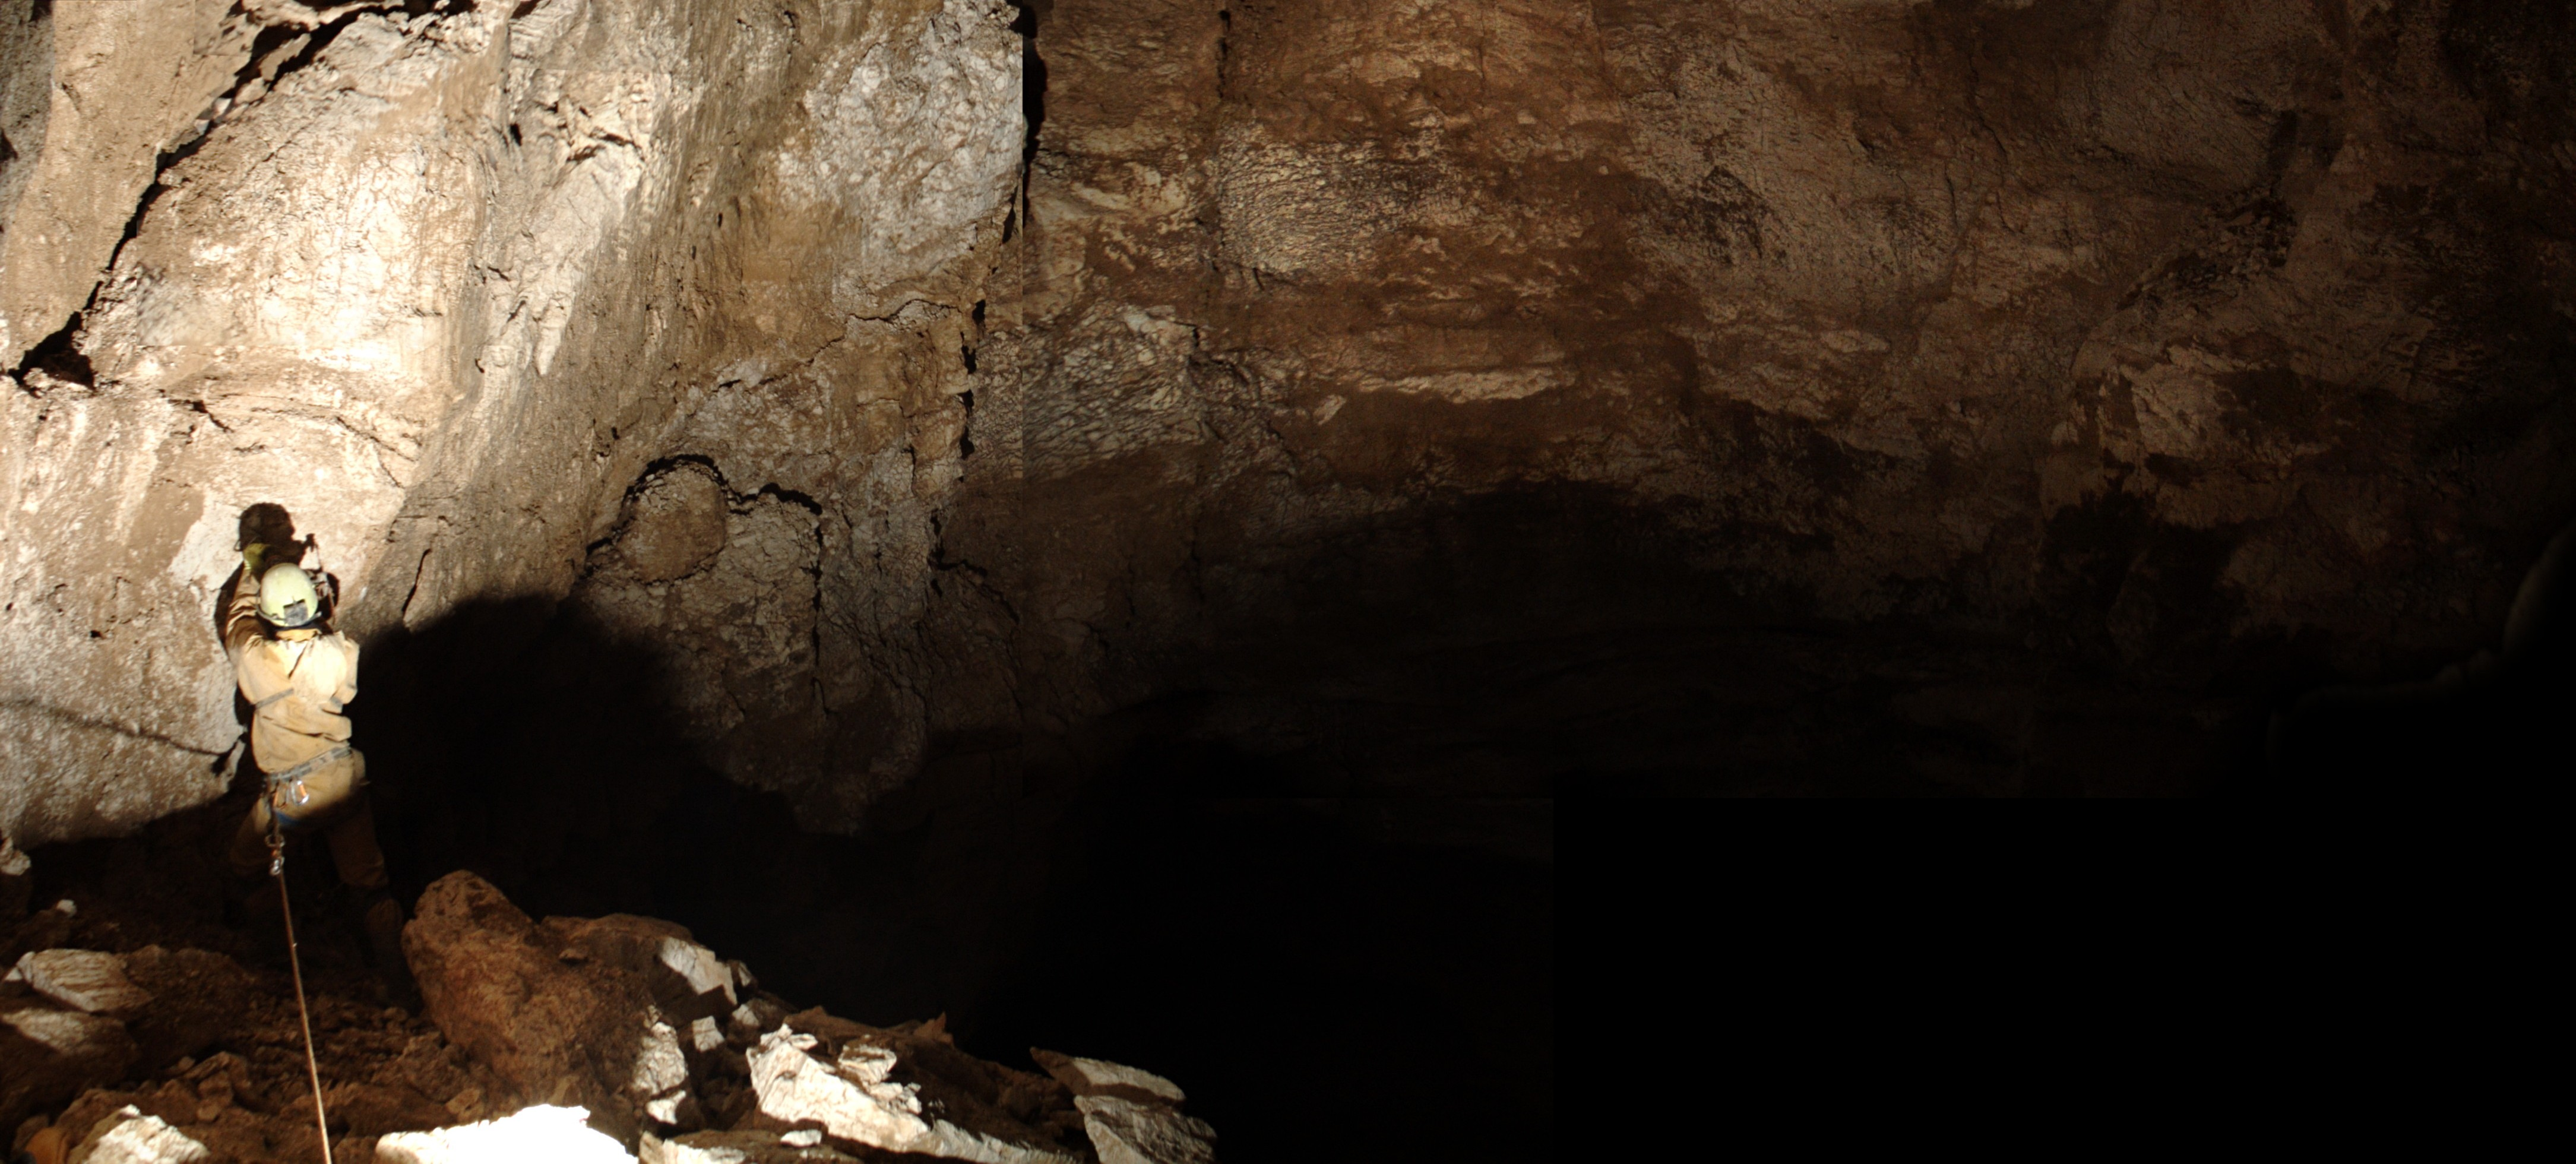
\includegraphics[width=\linewidth,]{2009/logbook/2009-08-10-20.51.38 - Jarvist Frost - Canon Powershot G5 - walk the line composite--orig.jpg}}
		\caption{}\label{gergely walk the line}
	\end{subfigure}

         \caption{The \protect\passage{Captain Kangaroo} branch continued down beyond \protect\passage{Dark Tranquillity}.
   		\textit{(a)} The 30 m high \protect\passage{Mirage Canyon}
     		\textit{(b)} Gergely bolting underneath limestone fluting at \protect\passage{2 Minutes to Midnight}, a 35 m pitch
     		\textit{(c)} Gergely continuing to bolt, now in \protect\passage{I walk the line}. \pic{Jarvist Frost}
		}
\end{pagefigure}